\documentclass[12pt]{article}
\usepackage{geometry} % to change the page dimensions
\usepackage{graphicx} % to include images
\usepackage{hyperref} % for hyperlinks
\usepackage[backend=biber,style=apa]{biblatex}

% Adjust the page margins
\geometry{a4paper}

\title{
    \textbf{Final Project Milestone: \\Daily Water Demand Forecasting} \\
    \vspace{0.5em}
    \large Project Category: General Machine Learning
}

\author{
    Haocheng Fan, hfan11 \\
}

\date{\today}

\begin{document}
\maketitle

\section*{Motivation}
My hometown, Shaoxing, is often called the "Eastern Venice" of China. But nowadays, we face big challenges in managing our water. With more people and changing weather patterns, 
it's getting harder to make sure we have enough water for everyone. As we use more technology and our population grows, our water needs become more complex. It's important for us to 
find solutions to these problems. We're looking into how machine learning can help us predict daily water needs so we can use our water wisely.

\section*{Preliminary Experiments}
\begin{enumerate}

    \item \textbf{Data Collection:}\\
    Due to the difficulties of data collection in China, we decide to find the similar region in population and climate parameter. Finally We sourced the dataset from IEEE dataport. It is the subtropical humid 
    region in Pakistan, with the similar average temperature and latitude as Shaoxing. This includes the daily data for water consumption, date, average temperature, average dew point, humidity, average precipitation.
    This enables us to do the daily water consumption forecasting. 


    \item \textbf{Data Pre-processing:}
    \begin{itemize}
        \item Construct the Correlation matrix to see the reasonable variables for the models:\\
        \begin{figure}[htb!]
            \centering
            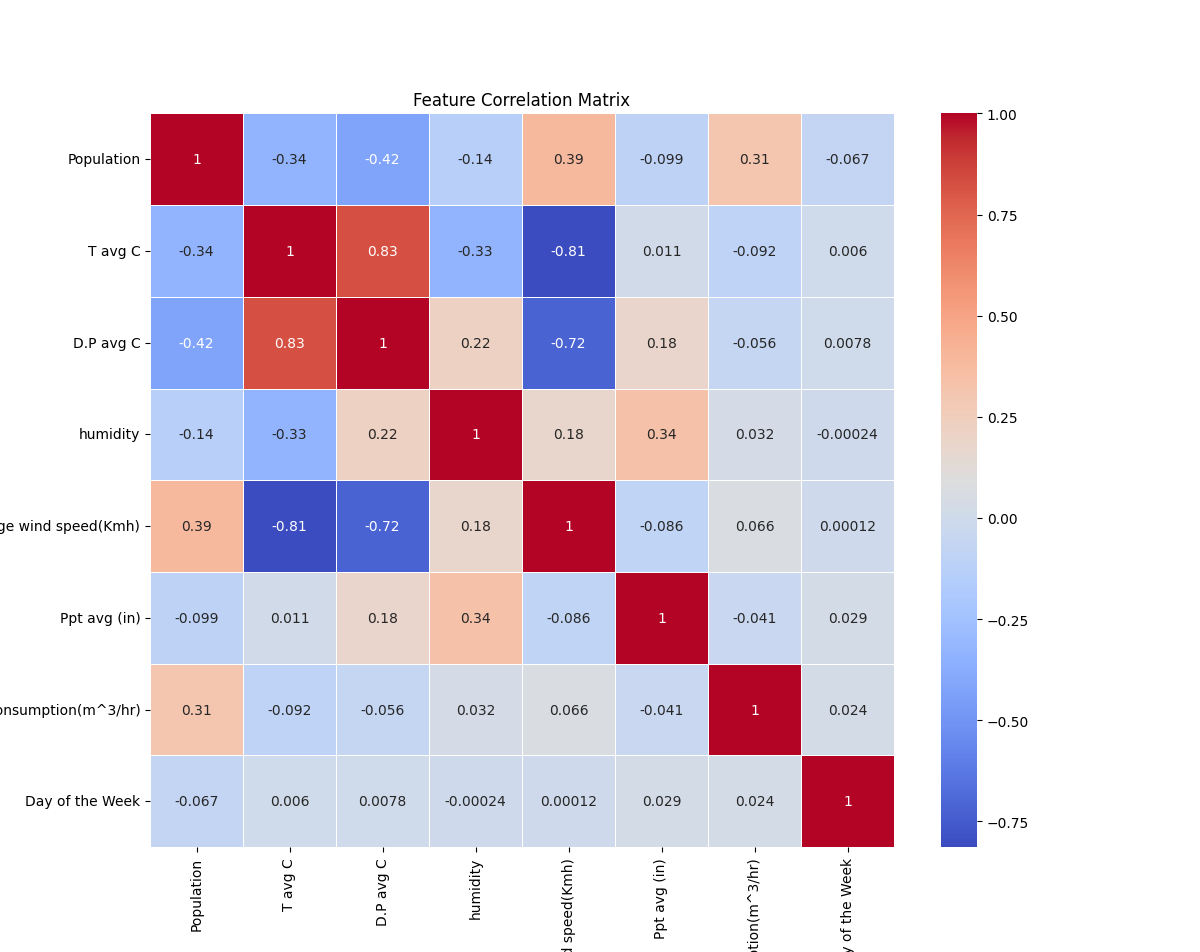
\includegraphics[width=0.75\linewidth]{C:/Users/Haoch/Desktop/cs229-project/milestone/correlation matrix.png}
            \caption{Correlation Matrix }
            \label{fig:Correlation}
        \end{figure}
        \item Select reasonable variables for the models: Figure 1 shows the correlation heatmap. It can be refered that the population have the maximum impact as they have 
        the maximum positive correlation with water consumption. Humidity, wind speed and day of the week also have the positive impact although the correlation is small. Therefore,
        the major parameter is population and the others are used to improve accuracy. 
        \item Analysis the water consumption related to the population. To clean the outlier data, we use the IQR method. Then we get the cleaned data to process to the training Model.
    \end{itemize}

    \item \textbf{Model Preparation and Training:}\\
        Set up the three machine learning model algorithms: Linear Regression (Baseline), Random Forest, and Support Vector Regression Model. We use 80 $\%$ as train set and 20$\%$ as validation set.\\

    \item \textbf{Model Evaluation:}
    \begin{itemize}
        \item Linear Regression Model:\\
        \begin{table}[h]
            \centering
            \begin{tabular}{|c|c|}
            \hline
            \textbf{Metrics} & \textbf{LR} \\
            \hline
            R$^2$ & [0.482] \\
            \hline
            MSE & [1010268] \\
            \hline
            MAE & [815.85] \\
            \hline
            \end{tabular}
            \caption{Metrics for Linear Regression (LR)}
            \label{tab:metrics_lr}
            \end{table}
        \item Random Forest Model:\\
        \begin{table}[h]
            \centering
            \begin{tabular}{|c|c|}
            \hline
            \textbf{Metrics} & \textbf{RF} \\
            \hline
            R$^2$ & [0.357] \\
            \hline
            MSE & [1228537] \\
            \hline
            MAE & [901.55] \\
            \hline
            \end{tabular}
            \caption{Metrics for Random Forest (RF)}
            \label{tab:metrics_lr}
            \end{table}
        \item Support Vector Regression Model:\\
        \begin{table}[h]
            \centering
            \begin{tabular}{|c|c|}
            \hline
            \textbf{Metrics} & \textbf{SVR} \\
            \hline
            R$^2$ & [0.379] \\
            \hline
            MSE & [1169332] \\
            \hline
            MAE & [881.64] \\
            \hline
            \end{tabular}
            \caption{Metrics for Support Vector Regression Model (SVRM)}
            \label{tab:metrics_lr}
            \end{table}
    \end{itemize}

    \item \textbf{Error Analysis and Future Work:}\\
    Our results aren't as good as we hoped. When we look at our graphs, small changes in population can cause big changes in water use. 
    This makes it hard to train our model. We didn't have enough time to clean our data as much as we wanted.\\
    In future iterations of this project, we aim to investigate data decomposition methods, such as PCA and SVD, 
    to better discern underlying patterns and potentially reduce the influence of noise in our dataset. If you have any better ideas, please let me know.\\

\end{enumerate}
    


\section*{References}
Q, Shuang \& Zhao, RT. (2021). Water Demand Prediction Using Machine Learning Methods: A Case Study of the Beijing–Tianjin–Hebei Region in China. \textit{Water}, 13(3), 310. https://doi.org/10.3390/w13030310.\\


Kavya, M., Mathew, Aneesh, Shekar, Padala Raja & Sarwesh, P. (2023). Short term water demand forecast modelling using artificial intelligence for smart water management. \textit{Sustainable Cities and Society}, 95, 104610. https://doi.org/10.1016/j.scs.2023.104610.



\end{document}
